\documentclass{article} % For LaTeX2e
\usepackage{nips, times}
\usepackage{hyperref}
\usepackage{url}
\usepackage{subfig}

\usepackage{graphicx}
\usepackage{amsmath}
\usepackage{amssymb}
\usepackage{booktabs}
\usepackage{tabularx}
\usepackage{caption}
\usepackage{subcaption}
\usepackage{color}
\usepackage{relsize}
\usepackage{placeins}
\usepackage{natbib}
\usepackage{paralist}

\renewcommand{\null}{\operatorname{null}}
\newcommand{\given}{\,|\,}

\input math.tex

\newcommand{\OO}{\mathcal{O}}
\newcommand{\RR}{\mathcal{R}}

\nipsfinalcopy

\begin{document}
\title{Compressed Sensing for Traffic Networks}

\author{
Philipp Moritz\\
University of California\\
Berkeley, CA 94720, USA\\
\texttt{pcmoritz@eecs.berkeley.edu}\\
\And
Richard Shin\\
University of California\\
Berkeley, CA 94720, USA\\
\texttt{ricshin@eecs.berkeley.edu}\\
\And
Cathy Wu\\
University of California\\
Berkeley, CA 94720, USA\\
\texttt{cathywu@eecs.berkeley.edu}\\
\And
Fanny Yang\\
University of California\\
Berkeley, CA 94720, USA\\
\texttt{fanny-yang@eecs.berkeley.edu} \\
}

\maketitle

\begin{abstract}
Reconstructing true parameters from a partially observed model is a fundamental problem in science and technology.
In the last years there has been a surge of interest in this task under a broad variety of model assumptions.
Motivated by applications in traffic reconstruction, we investigate when blocks of probability distributions can be recovered from linear measurements.
We empirically study the performance of several reconstruction methods and review the literature on provably correct methods for the reconstruction of probability measures.
We evaluate several possible regularizers that can be used if the usual $\ell^1$ reconstruction is not applicable, because probability distributions have a built in $\ell^1$ constraint.
\end{abstract}

\section{Introduction}
The problem of estimating traffic demands between areas or along routes within a city from traffic counts on links in a network is an important problem in transportation planning. Good traffic demand estimates improve a road network's efficiency, reliability, and safety by a more effective use of its infrastructure. This problem been studied extensively in the transportation literature. One of the main challenges of this problem is the shortage of data needed for management of transportation networks, 

\begin{itemize}
\item traffic as a motivating problem
\item other applications
\item 
\end{itemize}

One of the main challenges of ICM projects is the shortage of data needed for management
of the transportation network. While traffic speed data and travel time estimates are increasingly more available from commercial vendors, they do not provide information about traffic volumes needed for effective traffic control, demand management and performance evaluation. Traffic vol-
25 umes are measured by static sensors, such as loop detectors, mounted into the infrastructure, and those are sparse. What helps in this situation is the knowledge of origin-destination (O-D) matrix and the information about route assignment.


\paragraph{Related work.}
Applications aside from traffic, e.g.

Existing techniques for traffic demand estimation.

Compressed sensing


Cite a lot of stuff

\section{Problem formulation and relaxations}
\begin{table}[htbp]
\caption{Notation for the traffic estimation problem}
\label{tab-notation}
\centering
\begin{tabular}{cl}
\toprule
Notation & Description \\
\midrule
$\OO$ & Set of origins. Its size $|\OO|$ is the number of zones. \\
$\RR$ & Set of all routes $r\in \RR$\\
$\RR^\gamma \subset\RR$ & Subset of routes starting at origin $\gamma\in\OO$ \\
$\RR^{\gamma \lambda} \subset\RR$ & Subset of routes from $\gamma\in\OO$ to $\lambda\in \OO$ \\
$b^\gamma$ & Flow (vehicle count) measured at origin $\gamma\in\OO$ \\
$n_\gamma$ & Number of routes from origin $\gamma\in \OO$\\
$x_\gamma \in[0, 1]^{n_\gamma}$ & $x_{\gamma r}$ is the portion of flow $b^\gamma$ directed to route $r \in \RR^\gamma$ \\
$A_{\gamma}$ & Corresponding blocks of $n_{\gamma}$ columns of $A$\\
\bottomrule
\end{tabular}
\end{table}

\paragraph{Losses.} (do we need to define these?)
$l(\alpha, \hat\alpha) = \norm{\hat\alpha - \alpha}_2$ & Loss/error of the estimated split vectors $\alpha$ in $\ell^2$ norm
$l'(\alpha, \hat\alpha) = \norm{\hat\alpha - \alpha}_1$ & Loss/error of the estimated split vectors $\alpha$ in $\ell^1$ norm
$l^*(\alpha, \hat \alpha) = \sum_{i}|1_{(\hat{\alpha}_i > 0)} - 1_{(\alpha_i > 0)}|.$ & Loss/error of the estimated split vectors $\alpha$ with respect to support recovery

\subsection{Mathematical modeling}
\begin{equation}\label{l0-minimization}
  \begin{split}
    \text{minimize} &\quad \norm{x}_0\\
    \text{subject to} &\quad Ax = b,\quad x\geq 0\quad \text{and}\quad 1^\T x_{\gamma} = 1\quad \forall \gamma=1,\dots, b
  \end{split}
\end{equation}

\subsection{One block relaxations}
We first consider the one-block case $\gamma = 1$. 
This problem can be solved if the original signal is the unique sparse solution. The following theorem gives conditions when this is the case. To show that the original vector is actually the unique sparsest one, we use the following theorem from \cite{Dahmen_CS}.
\begin{theorem}
\label{thm:l0unique}
Let $A \in \R^{m\times n}$ and $x\in\R^n$ be $s$-sparse. In the case
$m\geq 2k$, the problem $Ax = b$ can be recovered if and only if
\begin{inparaenum}[(a)]
\item the set $\Sigma_{2k}$ of $2k$-sparse vectors intersects with the null space of the matrix $A$ only at the singleton $\{0\}$ (see also section 2 of \cite{Dahmen_CS}).
\item For any subset $S$ with $|S| = 2k$, the matrix $A_S$ has rank $2k$ and
\item $A_S^\T A_S$ is invertible.
\end{inparaenum}
\end{theorem}
For deterministic matrices this is hard to check.

However this program is not solvable in polynomial time because it is combinatorically hard problem.Therefore in the past decade there has been a lot of work done linked to Compressed Sensing in order to come up with convex relaxations of the $\ell^0$ norm minimization which the $\ell^1$ norm minimization and to find conditions for which solving the approximation/relaxation work.
\begin{equation}\label{l1-minimization}
  \begin{split}
    \text{minimize} &\quad \norm{x}_1\\
    \text{subject to} &\quad Ax = b,\quad x\geq 0
  \end{split}
\end{equation}
In the matrix

Such conditions are for example the necessary and sufficient (Restricted) Nullspace property/restricted eigenvalue property and the sufficient restriced isometry property. For deterministic matrices these are not checkable in polynomial time, see \cite{DonohoCheckable}. But for random matrices with Gaussian entries this holds with high probability. For deterministic measurement matrices as in the case of our traffic matrices, there are other conditions like mutual coherence, see e.g. \cite{Fuchs}, which are much easier to check.

\begin{theorem}[Incoherence]
\end{theorem}

However our matrices are not incoherent. Also, note that in our case of a positive vector which sums to one, i.e. the $\ell^1$ constraint is already known. Unless the $k$-sparse probability measure $x^*$ is the unique solution of \eqref{l1-minimization}, we thus have to come up with a different regularization scheme to achieve strong recovery results. In the literature, this problem has been discussed as recovering probability measures. 

In \cite{mert} it was observed that for probability measures $x$ we have $1 = \norm{x}_1 \leq \norm{x}_0\cdot \norm{x}_\infty$ and thus $\norm{x}_{\infty}^{-1}$ is a lower bound on the size of the support of $x$. This suggests trying to use the inverse $\ell^\infty$ norm as a proxy for sparsity.
\begin{equation}\label{l8-minimization}
  \begin{split}
    \text{minimize} &\quad \frac{1}{\norm{x}_\infty}\\
    \text{subject to} &\quad Ax = b,\quad x\geq 0\quad\text{and}\quad 1^\T x = 1
  \end{split}
\end{equation}

Let $p^*$ denote the minimum value of $\norm{x}_0$ over $Ax = b$, we then consider the relaxation
\begin{equation}\label{l8-recovery}
  \begin{array}{rcllllr}
  p^* \geq& p_\infty^* &= \min\limits_x\, \norm{x}_\infty^{-1}&\text{such that $Ax = b$, $1^\T x = 1$}\quad \text{and}\\[5pt]
  &1/p_\infty^* &= \max\limits_{i=1,\dots,n} \max\limits_{x}\,x_i&\text{such that $Ax = b$, $1^\T x = 1$.}
  \end{array}
\end{equation}

\paragraph{Minimal cardinality selection.} Instead of taking the maximum over $1\leq i\leq n$ in the linear program formulation of \eqref{l8-recovery}

\subsection{Block probability recovery}
\subsection{Block $\ell^\infty$ regularization}
Instead of a single probability measure $x\in \R^n$, in the traffic
flow problem we are given blockwise probability measures $x = (x_1,
\dots, x_b)^\T$ where $1^\T x_\gamma = 1$ for all blocks $\gamma\in
\{1, \dots, b\}$. Define
\begin{equation*}
  \mathcal B_n^k = \{x = (x_1, \dots, x_b)^\T : x_\gamma \in \R_+^{n_\gamma}, \norm{x_\gamma}_0 = k_\gamma, \norm{x_\gamma}_1 = 1\text{ for $1\leq \gamma\leq b$}\},
\end{equation*}
where $n = (n_1, \dots, n_b)$ are the respective sizes of the blocks
and $k = (k_1, \dots, k_b)$ their sparsities. The minimum cardinality
reconstruction can then be formulated as
\begin{equation}
  \begin{split}
    &\text{minimize}\quad \norm{x}_0\\
    &\text{subject to}\quad Ax = b\quad\text{and}\quad x\in \mathcal B_n^k.
  \end{split}
\end{equation}
Similar to the $\ell^\infty$ relaxation in the one-block case, we can
relax this intractable problem to
\begin{equation}\label{block-relaxation}
  \begin{split}
    &\text{minimize}\quad \textstyle\sum_{\gamma=1}^b {\norm{x_\gamma}_\infty^{-1}}\\
    &\text{subject to}\quad Ax = b\quad\text{and}\quad x\in \mathcal B_n^k.
  \end{split}
\end{equation}



\section{Guarantees for sparse recovery}
To guarantee exact sparse recovery, the following procedure will be used: First, assuming that the original vector~$x^*$ is actually the sparsest solution to~\eqref{l0-minimization}. Then, we prove that the solution of the relaxed problems~\eqref{l1-minimization} and~\eqref{l8-minimization} are unique and equal to $x^*$.


\subsection{Obtaining the sparse solution by Compressed Sensing}
The convex relaxation of the original $\ell_0$-minimization problem
has been studied in many different settings by the Compressed Sensing
community.
The following elementary but particularly elegant (although not optimal) example was given by Benjamin Recht during the ``BigData Bootcamp'' at the Simons Institute in Berkeley.
\begin{theorem}
  Let $x^*\in \R^n$ be $s$-sparse and $A \in \R^{m\times n}$ be a
  random matrix with independent entries $A_{ij}\sim \text{N}(0,
  m^{-1})$. If $m \geq 2 (1+\epsilon) s\log n + s + 1$ then $x^*$ is
  the unique solution of
  \begin{align}
    &\text{minimize}\quad \norm{x}_1\label{CS}\\
    &\text{subject to}\quad Ax = Ax^* = b \nonumber
  \end{align}
  with probability at least $1 - 2\exp\bigl(-\bigl(\sqrt{(1+\epsilon)/(2s) +
      \epsilon} - \sqrt{(1+\epsilon)/(2s)}\bigr)^2\cdot \log n\bigr).$
\end{theorem}

With a stronger albeit less elegant technique than the one Ben used, the factor $\log n$ in the bound on the number of constraints can be improved to $\log(n/s)$.
%% TODO: Uniqueness
\begin{proof}
Let $S$ denote the support of $x^*$. The proof relies on the so called \emph{primal-dual witness} technique \cite{Wainwright2009}: We construct a pair of vectors that are primal and dual optimal and act as a witness for correct support recovery.
The following lemma formalizes the notion of a primal-dual witness $(x, \lambda)\in \R^{n\times m}$.
\begin{lemma}\label{l1-lemma}
  (a) A vector $x \in \R^n$ is optimal for \eqref{CS} if there exists
  a vector $\lambda\in \R^m$ such that $A^\T \lambda\in \partial
  \norm{x}_1$ and $Ax = b$ and (b) if the vector $v = A^\T \lambda$
  satisfies the strict dual feasibility condition $|v_j| < 1$
  for all $j\not\in S$, any optimal solution to \eqref{CS} satisfies
  $x_j = 0$ for all $j\not\in S$.
\end{lemma}
The proof is immediate: The problem \eqref{CS} is solved by $x\in
\R^n$ if and only if $\norm{x + h}_1 \geq \norm{x}_1$ for all $h\in \null(A)$.
The latter condition is true if there is a $\lambda \in \R^m$ such
that $A^\T \lambda \in \partial \norm{x}_1$ and $Ax = b$, because from
the subgradient condition we can then for all $h\in \null(A)$ conclude
\begin{equation*}
\norm{x + h}_1 \geq \norm{x}_1 + \sprod{A^\T \lambda, h} = \norm{x}_1 +
  \sprod{\lambda, A h} = \norm{x}_1.
\end{equation*}
The second part immediately follows from $v \in \partial\norm{x}_1$,
thus $v_j \in \{+1, -1\}$ if $x_j \neq 0$. \qedhere

Back to the main proof, we thus have to construct a Lagrange multiplier $\lambda$ such that $v = A^\T \lambda$ and $v_k = \sign(x^*_k)$ if $x^*_k\neq 0$ and $|v_k| < 1$ otherwise. Let $S$ be the support of $x^*$, then we define $e = \sign(x^*_S)\in \R^s$. Our task is then to find $\lambda$ such that
\begin{align}\label{compressed_equation}
  (A^\T \lambda)_S = e\quad\text{and}\quad \norm{(A^\T \lambda)_{S^c}}_\infty < 1.
\end{align}
  We can assume that $A = (A_S, A_{S^c})$ and $x = (x_S, x_{S^c})^\T$. The strategy is to solve the first equation in~\eqref{compressed_equation} by least squares and then verify the second equation. The optimization problem that has to be solved is
  \begin{align*}
    &\text{minimize}\quad \norm{\lambda}^2\\
    &\text{subject to}\quad A_S^\T \lambda = e.
  \end{align*}
    Because $A$ is Gaussian and thus of full rank\footnote{this is in fact in general true for matrices with indices drawn i.i.d. from a continuous distribution}, the solution can be calculated using the Moore-Penrose pseudoinverse $\lambda = A_S(A_S^\T A_S)^{-1} e$.
It remains to show that for $z = A_{S^c}^\T\lambda$ the $l^{\infty}$ norm is strictly smaller than $1$ with high probability. First observe that $\|\lambda\|^2 = e^\T(A_S^\T A_S)^{-1} e$.
From this it follows\footnote{if $x_k \sim \operatorname{N}_p(0, \Sigma)$ is from a multivariate Gaussian and $X = (x_1, \dots, x_n)^\T \in \R^{n\times p}$, then $(X^\T X)^{-1} \sim W_p^{-1}(\Sigma^{-1}, n)$ is from an inverse Wishart distribution and therefore $z^\T (X^\T X)^{-1} z$ is an inverse $\chi^2$ variable with parameters $z^\T \Sigma^{-1} z/2$ and $(n-p+1)/2$.} that $\|\lambda\|^2\sim \text{Inv-$\chi^2$}((m-s+1)/2, m \norm{e}^2/2)$ where $\norm{e}^2 = s$. With the large deviation bound for the inverse $\chi^2$
\begin{align*}
  \P\left(\norm{\lambda} > \sqrt{\frac{ms}{m-s+1-t}}\right) \leq
  \exp\left(-\frac{t^2}{4(m-s+1)}\right)
\end{align*}
we get $\P(|z_k| > 1 \given \norm{\lambda} \leq
\sqrt{ms/(m-s+1-t)}) \leq \P(|w| > 1\given w\sim N(0, s/(m-s+1-t))
\leq \exp(-(m-s+1-t)/(2s))$ and therefore we have
\begin{equation*}
  \P(\norm{z}_\infty > 1) \leq (n-s)\cdot \exp\left(-\frac{m-s+1-t}{2s}\right) + 
  \exp\left(-\frac{t^2}{4(m-s+1)}\right).
\end{equation*}
Setting $t = 2(1+\epsilon) \cdot s\cdot \log n
\cdot (\sqrt{1-2s\epsilon/(1+\epsilon)} - 1)$ concludes the proof.\qed
    \end{proof}

\subsection{Recovery of sparse probability measures}
We will present two methods for the reconstruction of sparse probability measures:  Classical Lasso, regularization with the $\ell^\infty$ norm and minimal cardinality selection.

Since we always consider the case when our probability measures are sparse, one natural approach would be to use the classical Lasso - if our probability measure is the unique $k$-sparse solution to $Ax  = b$, then we can abandon the $\ell^1$ constraints and use classical $\ell^1$ regularization. Guarantees for random measurement matrices with Gaussian entries are given in the following.

It is well-known (\cite{inverse_problems}) that the $\ell^1$ relaxation in \eqref{l1-minimization} is an instance of the following more general problem 
\begin{equation}
\label{eq:MinAtomicNorm}
\min \|x\|_{\A} \:\: \text{ s.t. } Ax = b,
\end{equation}
where $\A$ is a set of atoms in $\R^n$ and $\|\cdot \|_{\A}$ represents the atomic norm defined as follows.
\begin{definition}[Atomic norm]
$\|x\|_{\A} = \inf\{ t>0: x\in t \conv(\A)\}$ is called the atomic norm of $x$ induced by $\A$ in case $\A$ is symmetric about the origin.
\end{definition}
Our case of minimization over sparse vectors using the $\ell^1$ norm can be retrieved from this definition by choosing $\A = \{\pm e_i: i = 1,\dots, p\}$ where $e_i$ are the canonical basis vectors in $\R^n$.

In order to examine recovery conditions the following definitions are useful:
\begin{definition}[Tangent cone]
The tangent cone at $x$ is defined as 
\begin{equation}
\label{eq:TangentCone}
T_{\A}(x) = \cone \{\hat{x} - x: \|\hat{x}\|_{\A} \leq \|x\|_{\A}\}
\end{equation}
\end{definition}
The tangent cone is the set of directions at $x$ for which the atomic norm decreases. Therefore, whenever the null space of $A$ and $T_{\A}(x^*)$ do not intersect, $x^*$ minimizes \eqref{eq:MinAtomicNorm}. To bound this probability, we introduce the following theorem.

\begin{theorem}
\label{thm:ExpectationBound}
Let $\Omega$ be a closed subset of $\mathbb{S}^{n-1} = \{x: \|x\|_2 = 1\}$ and $A$ be a matrix with i.i.d. zero-mean Gaussian entries having variance one. Then
\begin{equation}
  \EE \left[ \min_{x\in \Omega} \|A x\|_2 \right] \geq \lambda_n - w(\Omega)
\end{equation} 
where $n/\sqrt{n+1} \leq \lambda_n\leq \sqrt{n}$ and $w(\Omega)$ is the \emph{Gaussian width}
$w(\Omega) = \EE_{g} \left[ \sup_{z\in \Omega} \sprod{g, z} \right]$
\end{theorem}

The difference between problem~\eqref{eq:MinAtomicNorm} and \eqref{l1-minimization} is that we have an additional constraint of the form $1^\T x = 1$.
With $\mathcal P = \{ x: 1^\T x = 1 \text{ and }0\leq x\leq 1\}$ we can thus write our problem as
\begin{equation}
\label{eq:MinAtomicNorm_ProbSimplex}
\min \|x\|_{\A} \:\: \text{ s.t. } Ax = b \text{ and } x\in \mathcal P.
\end{equation} 
Using Theorem \ref{thm:ExpectationBound} and the definitions therein we can then extend Corollary 3.3 in \cite{inverse_problems} and get the following result.
\begin{theorem}
\label{thm:UniqueRecovery}
  Let $A\in \R^{m\times n}$ be a random matrix with independent
  entries $A_{ij}\sim N(0, 1)$ and let $\Omega = \mathcal P \cap T_{\mathcal
    A}(x^*)\cap \mathbb{S}^{n-1}$. Suppose that we have
  measurements $b = Ax^*$. Then $x^*$ is the unique optimum of
  \eqref{l1-minimization} with probability at least $1 - \exp(-\frac 1
  2 (\lambda_n - w(\Omega))^2$ if we have $m\geq w(\Omega)^2 + 1$
  constraints.
\end{theorem}

 The proof is unchanged compared with \cite{inverse_problems}: We bound $\P(\min_{x\in \Omega} \|A x\|_2 >0)$ by using the result in Theorem \ref{thm:ExpectationBound}. This does not change by adding the closed constraint set $\mathcal P$. Using these preparations we can now state the major guarantee:
\begin{theorem}
If $m\geq 4k\log n$ we can recover $x^*$ by solving \eqref{eq:MinAtomicNorm_ProbSimplex} with high probability.
\end{theorem}
\begin{proof}
\footnote{from personal communication with Mert Pilanci}
Using Theorem \ref{thm:UniqueRecovery} we only need to calculate $w(\Omega)$. First define $S$ as the support of $x^*$. The tangent cone then consists of vectors $z = \hat{x} - x^*$ where $\hat{x}$ is a feasible solution. Then $z_{S^c} \geq 0$ and $\sum_{i=1}^n z_i = 0$, which implies $\|z_{S^c}\|_1 = \sum_{i\in S^c} z_i = -\sum_{i\in S} z_i \leq \norm{z_S}_1$. It follows that
\begin{equation*}
\|z\|_1 \leq \|z_{S^c}\|_1  +\|z_S\|_1 \leq 2 \|z_S\|_1 \leq 2\sqrt{k} \|z\|_2 = 2\sqrt{k},
\end{equation*} 
in the last step we used $\|z\|_2=1$ on $\Omega$. Using H\"older's inequality, the Gaussian width can be bounded by
\begin{equation}
w(\Omega) = \EE_g \left[ \sup_{z}\, \sprod{g, z} \:\:  \text{ s.t. } \|z\|_1 \leq 2\sqrt{k} \right] \leq 2\sqrt k\cdot \E_g \left[\sup_z\,\norm{g}_\infty\right].
\end{equation}
The term $\E_g[\norm{g}_\infty]$ can be bounded in the following way.
For $g\sim N(0, 1)$ we have $\P(|g|>t) \leq 2e^{-t^2/2}$ and therefore $\P(\max_{1\leq i\leq n} |g_i| > t) \leq 2ne^{-t^2/2}$. Therefore, we get
\begin{equation*}
  \E_g[\norm{g}_\infty] \leq x + 2n\int_{t=x}^\infty e^{-t^2/2}\,\d t
  \leq x + 2n\cdot \frac 1 x \cdot e^{-x^2/2}.
\end{equation*}
Choosing $x = \sqrt{2\log n}$ yields $\E_g[\norm{g}_\infty] \leq
\sqrt{2\log(n)} + 2$.

Then we could use Theorem \ref{thm:UniqueRecovery} and obtain $m\geq  w(\Omega)^2 + 1$.\\
\end{proof}

After establishing the guarantees for the Lasso approach, the question now is whether we can improve them, i.e. need smaller amount of measurements while maintaining the same probability of recovery. This seems intuitively possible since we are given one additional sum to one constraints, i.e.an additional measurement. 

\paragraph{Regularization with the $\ell^\infty$ norm.} If the vector $x^*$ to be recovered is a sparse probability measure, the technique described in the previous section is not applicable, because $\norm{x}_1 = 1$ for probability measures.

%% Vandermonde matrix: if min card(x) unique, then recovery, not for L1

%% Boyd, Candes: reweighted L1, gives the card-approximation

%% Sahan, Negaban + martin: unified framework for M-estimators

%% \cite{foygel}

\subsection{Recovery of sparse block probability measures}



??? Transition needed ???

This reconstruction procedure may seem suboptimal, because it does not
take into account the block structure of our measurements.
However, knowledge of this structure does not help much in our situation as we
argue now. The number of measurements needed for reconstruction in
compressed sensing is typically of the order
$\O(k\log(n/k))$.
Intuitively, the first factor specifies the number
of measurements necessary to recover the $k$ nonzero entries of the
true parameter and the second factor is the number of measurements
needed for estimating the right support. If we have constraints on the
support, we can use a technique like \emph{model-based compressed
  sensing} \cite{model_sensing} to reduce this second factor.  
Let $m_k$ be the number of possible support configurations with
sparsity $k$, then with a model-based approach we need on the order or
$\O(k\log(m_k))$ measurements.
For $m_k = {n\choose k}\approx (ne/k)^k$, we recover the compressed
sensing result.
In our case, if we have $b$ blocks of size $\nu$ each, each with
sparsity $\kappa$ (thus $n = b\nu$ and $k=b\kappa$), we get
\begin{equation*}
m_k = {\nu \choose \kappa}^b \approx \left(\frac{\nu
  e}{\kappa}\right)^{b\kappa} = \left(\frac{ne}{k}\right)^k,
\end{equation*}
which is the same result as above. The interpretation of this is that
the support configurations that violate the block assumption are a
negligible portion of all the possible support configurations.


\section{Algorithms for reconstructing block probability measures}
\subsection{Entropy minimization}
For a discrete random variable $X$ with values in $\{1, \dots, n\}$ and probabilities $\P(X = k) = p_k$, the entropy is defined as $H(X)  = -\sum_{i=1}^{n} p_i \log p_i$.
Intuitively, a random variable with a sparse probability measure has a more unpredictable value, and therefore lower entropy (in particular, if the random variable has only one possible outcome, then the entropy is 0).
In addition, entropy provides a lower bound on the cardinality of a probability distribution. When $\|x\|_0 = n$, then maximum entropy $H(x) = \log n$ is attained when the $n$ non-zero possibilities have equal weight and therefore $H(x) < \|x\|_0$.

We provide the following argument for why it may be preferable to optimize for entropy instead of the $\ell_\infty$ norm.
Consider the probability distribution $p = (0.5, 0.5, 0)$ over three discrete possibilities.
If we use $\norm{p}_{\infty}^{-1}$ as the criterion to optimize, then all distributions where one of the entries remains $0.5$ are equally preferred.
With entropy, as we increase $p_3$, one of $p_1$ or $p_2$ must increase correspondingly; for example, $q = (0.7729, 0.1135, 0.1135)$ has the same entropy as $p$.
This seems to better fit our assumption that most people from each origin will go to a small number of destinations, which is why we desired sparsity in the first place.

In entropy minimization, we attempt to solve the following:
\begin{align*}
&  \min_{x} \sum_\gamma H(x_\gamma) \qquad \text{ s.t. } Ax = b, \sum_i x_{\gamma, i} = 1\ \forall \gamma \\
=& \min_{x} \gamma H(x) \qquad \text{ s.t. } Ax = b, \sum_i x_{\gamma, i} = 1\ \forall \gamma
\end{align*}
%This problem also allows us to distinguish between multiple solutions which have the same cardinality, since two solutions which are not exactly the same will have different entropy.
Unfortunately, $H(X)$ is a concave function, so the above is a concave minimization problem, albeit with a convex set as the constraint.
However, as $H(X)$ is differentiable, we can still use a first-order gradient descent method for constrained problems (without any guarantees on optimality) in the following way:
\begin{enumerate}
  \item Find a feasible $x$, i.e., which satisfies $Ax = b, \sum_i x_{\gamma, i} = 1$ for all $\gamma$.
  \item Compute the gradient of the objective function at $x_0$.
  \item Find a feasible update direction $\Delta x$, selected to minimize the dot product between it and the gradient.
  \item Find $\alpha \le 1$ so that $H(x + \alpha \Delta x) < H(x)$. If no such $\alpha$ exists, terminate.
  \item Update $x_\textrm{new} = x + \alpha \Delta x$, and repeat the above steps.
\end{enumerate}
\cite{sudoku} describes a similar method for entropy minimization, but they take additional steps to try to escape local minima, by occasionally updating $x$ to increase entropy instead of decreasing it.

\subsection{Random sampling}
The objective in \eqref{block-relaxation} can be rewritten as
$\sum_\gamma \norm{x_\gamma}_\infty = \sum_\gamma (\max_i\,x_{\gamma
  i})^{-1} = \min_{(i_1, \dots, i_b)} \sum_\gamma x_{\gamma i_\gamma}$.
Optimizing it over $\mathcal C = \mathcal B_n^k \cap \{x : Ax =
b\}$ we get
\begin{equation*}
  p_\infty^* = \min_{i_1, \dots, i_p} \min_{x\in \mathcal C}\,
  {\textstyle \sum_\gamma x_{\gamma i_\gamma}},\quad
  \text{or equivalently}\quad
  (p_\infty^*)^{-1} = \min_{i_1, \dots, i_p} \max_{x\in \mathcal C} \,
  {\textstyle \sum_\gamma x_{\gamma i_\gamma}}.
\end{equation*}
The minimum is now over exponentially many configurations and thus
computationally intractable. We suggest to use a random sampling
strategy: Get a pilot estimate $\check x$ for $x^*$, for example by
minimizing the $\ell^1$ norm or the elastic net over all $x$ with $Ax
= b$ (without the block probability constraints). Then, random
sampling proceeds as follows:
\begin{enumerate}
  \item 
\end{enumerate}

\section{Numerical Results}

To test our algorithms, we generated two datasets: One to assess reconstruction performance on the traffic estimation problem and one to empirically evaluate the theoretical guarantees from section \ref{sec:theory}.
\begin{figure}
  \subfloat[][Small road network with weights]{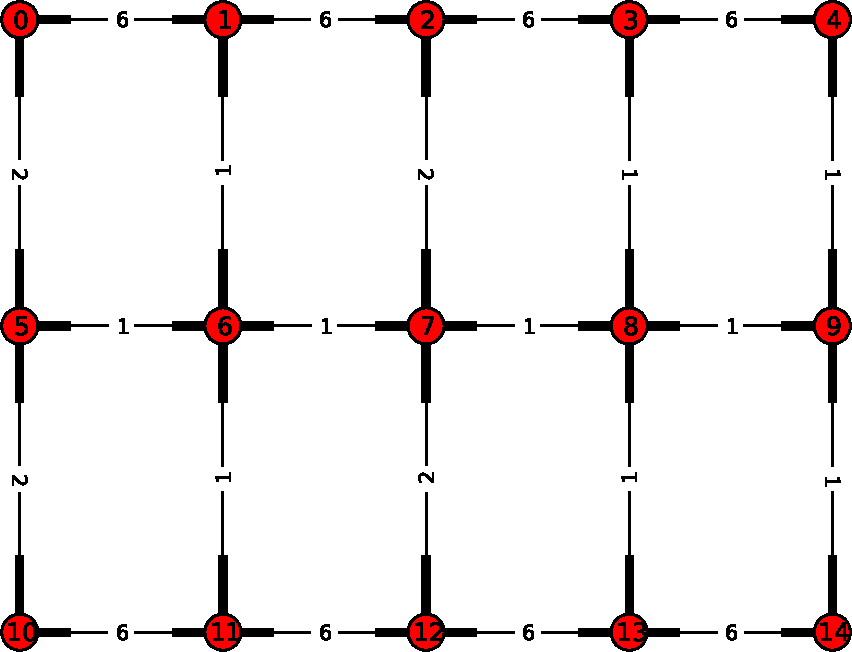
\includegraphics[width=0.4\textwidth]{figures/small-graph.pdf}}
  \qquad
  \subfloat[][Flows for the small network]{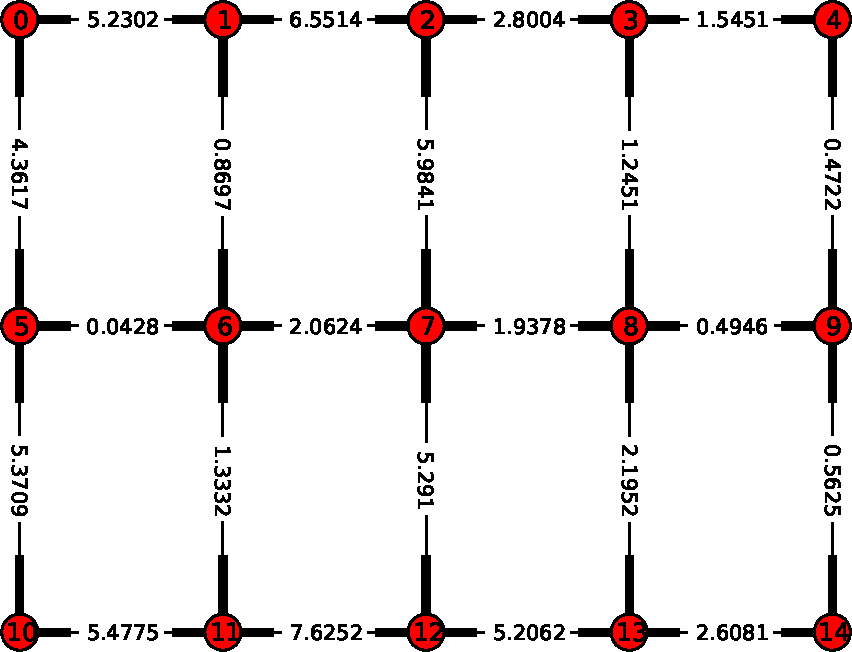
\includegraphics[width=0.4\textwidth]{figures/small-flow.pdf}}
  \caption{A traffic graph for $r=3$ and $c=5$. As shown in (a), there are horizontal highways with weight $6$ at the top and the bottom. These are vertically connected by roads with weights 1 or 2. In (b), the flows on these roads were computed by first choosing the $k$ shortest paths between each origin-destination pair. Then, for each origin $u$, we choose $s$ of the shortest paths starting at $u$ uniformly at random. These are endowed with a draw from Dirichlet with parameter $(1, \dots, 1)\in \R^s$}
\end{figure}
\paragraph{Traffic matrices.} The parameters for this model are the number of rows $r$ and the number $c$ of columns in the road grid and the number $k$ of routes per origin-destination pair, the sparsity $s$ and the flow from each node $\phi$.
\paragraph{Gaussian random matrices.} The parameters are: Sparsity $k$, number of blocks $b$, number of variables per block $\nu$ and number of measurements $m$.
First, a vector $x^*\in \mathcal B_n^s$ with $n = (\nu, \dots, \nu)$ and
\begin{equation*}
s = (\lfloor k/\nu\rfloor + \alpha_1, \dots, \lfloor k/\nu\rfloor + \alpha_b)\quad\text{with $\alpha_i = 0, 1$ such that $k = b\cdot \lfloor k/\nu\rfloor + 1^\T \alpha$.}
\end{equation*}
is generated by choosing $x_\gamma \sim \operatorname{Dirichlet}(1,
\dots, 1)$ on the support of $x_\gamma$ as determined by $\mathcal
B_n^s$ for $\gamma = 1, \dots, b$. Then we choose a Gaussian random matrix $A\in \R^{m\times |n|}$ with unit variance.

\section{The code}
Our code is available at \url{https://github.com/pcmoritz/traffic-project}. It consists of the following modules:
\begin{enumerate}
  \item The algorithms are implemented in
    \begin{itemize}
      \item \texttt{cvx\_L2}
      \end{itemize}
\end{enumerater}

\section{References}

\FloatBarrier
\vskip 0.2in
\nocite{*}
\bibliographystyle{plain}
\bibliography{lit}
\end{document}
